\documentclass{article}
\usepackage{CJKutf8}
\usepackage{graphicx}
\usepackage{amsthm}
\let\proof\relax \let\endproof\relax % 避免 math_blog 重复定义 proof 报错
\usepackage{math_blog}
\usepackage{amsmath}
\usepackage{amssymb}
\usepackage{appendix}
\usepackage[normalem]{ulem}
\usepackage[thicklines]{cancel}
\usepackage{tikz}
\usetikzlibrary{positioning,arrows.meta}
\usepackage{pgfplots}

% Defensive: resolve possible \proof / theorem-env conflicts with math_blog
\makeatletter
\@ifundefined{proof}{}{\let\proof\@undefined \let\endproof\@undefined}
\@ifundefined{theorem}{\newtheorem{theorem}{Theorem}[section]}{}
\@ifundefined{lemma}{\newtheorem{lemma}[theorem]{Lemma}}{}
\@ifundefined{definition}{\newtheorem{definition}[theorem]{Definition}}{}
\@ifundefined{proposition}{\newtheorem{proposition}[theorem]{Proposition}}{}
\@ifundefined{corollary}{\newtheorem{corollary}[theorem]{Corollary}}{}
\@ifundefined{remark}{\newtheorem*{remark}{Remark}}{}
\@ifundefined{example}{\newtheorem*{example}{Example}}{}
\makeatother
\newenvironment{proof}[1][证明]{%
  \par\smallskip\noindent\textit{\textbf{#1.}}\quad\ignorespaces
}{%
  \hfill$\square$\par\smallskip
}

% 中文环境名（与 theorem 共用计数器）
\theoremstyle{plain}
\newtheorem{zhtheorem}[theorem]{定理}
\newtheorem{zhlemma}[theorem]{引理}
\newtheorem{zhcorollary}[theorem]{推论}
\theoremstyle{definition}
\newtheorem{zhdefinition}[theorem]{定义}
\newtheorem{zhexample}[theorem]{例}
\theoremstyle{remark}
\newtheorem*{zhremark}{注}
\let\theorem\zhtheorem \let\endtheorem\endzhtheorem
\let\lemma\zhlemma \let\endlemma\endzhlemma
\let\corollary\zhcorollary \let\endcorollary\endzhcorollary
\let\definition\zhdefinition \let\enddefinition\endzhdefinition
\let\example\zhexample \let\endexample\endzhexample
\let\remark\zhremark \let\endremark\endzhremark
\renewcommand{\figurename}{图}
\renewcommand{\tablename}{表}
\renewcommand{\refname}{参考文献}
\numberwithin{equation}{section}

\title{[SDE V] 前向--倒向随机微分方程与随机极大值原理}
\author{Anqiao Ouyang}
\date{June 6, 2026}

\newcommand{\Title}{前向--倒向随机微分方程与随机极大值原理}
\newcommand{\Column}{Stochastic Differential Equations V}
\newcommand{\Author}{Anqiao Ouyang}

% Math shortcuts
\newcommand{\E}{\mathbb{E}}
\newcommand{\Prob}{\mathbb{P}}
\newcommand{\R}{\mathbb{R}}
\newcommand{\F}{\mathcal{F}}
\newcommand{\Lc}{\mathcal{L}}
\newcommand{\Sc}{\mathcal{S}}
\newcommand{\Hc}{\mathcal{H}}

\begin{document}
\begin{CJK*}{UTF8}{gbsn}

\maketitle

\section{引言}

在 [SDE~IV] 中我们发展了 BSDE 与非线性 Feynman--Kac 表示。那里的 Markov 情形有一个严格的结构：一个前向扩散 $X$，其系数 $(b,\sigma)$ 只依赖于 $(t,X_t)$，并与关于 $(Y,Z)$ 的倒向方程耦合，后者的驱动 $f$ 依赖于 $(t,X_t,Y_t,Z_t)$。关键在于，\emph{前向}系数感受不到 $Y$ 或 $Z$：BSDE 是骑在一个自治扩散之上的。

这种不对称并非巧合。正是它使得 Pardoux--Peng 的 Picard 压缩证明成为可能：$X$ 一次性被固定下来，只有 $(Y,Z)$ 在迭代。许多自然的问题打破了这种不对称。

\paragraph{引子例：带反馈的 LQ 控制。}
考虑 $[0,T]$ 上的线性--二次问题
\[
  dX_t=(AX_t+B\alpha_t)\,dt+\sigma\,dB_t,\qquad X_0=x,
\]
代价为
\[
  J(\alpha)=\E\!\left[\int_0^T\bigl(X_t^\top QX_t+\alpha_t^\top R\alpha_t\bigr)\,dt+X_T^\top GX_T\right].
\]
在上述代价约定下，Pontryagin 极大值原理（\S5）给出
\[
  \alpha_t^*=-\frac12 R^{-1}B^\top Y_t,
\]
其中 $Y$ 是伴随过程。把反馈代回状态方程，得
\[
  dX_t=\left(AX_t-\frac12 BR^{-1}B^\top Y_t\right)dt+\sigma\,dB_t.
\]
前向方程现在依赖于 $Y$ 了。于是 $(X,Y)$ 是真正耦合的：$X$ 把信息往前推，$Y$ 把信息往后推，而\emph{两者互相依赖}。这正是一个\textbf{前向--倒向随机微分方程}，即 FBSDE。

\paragraph{改变了什么。} [SDE~IV] 的解耦情形可以分两遍求解：先正向解 $X$，再倒向解 $(Y,Z)$。一个耦合的 FBSDE 没有这样的先后顺序；对整个三元组 $(X,Y,Z)$ 做不动点迭代未必收缩，因为前向误差会传入倒向方程，反之亦然。为处理这一点，已经出现了三种不同的技术：
\begin{itemize}
  \item \textbf{单调性方法。}对系数施加一个代数结构条件，在恰当的内积下恢复足够的耗散性。
  \item \textbf{小视域方法。}在足够短的时间区间 $[0,T]$ 上，压缩映射像解耦情形一样奏效。
  \item \textbf{四步格式。}当对应的非线性 PDE 有古典解时，从 PDE 构造 FBSDE 的解。
\end{itemize}

每种技术都照亮了同一对象的不同侧面。本文将：
\begin{itemize}
  \item 精确定义耦合 FBSDE，并指出朴素迭代的障碍（\S2）；
  \item 在 Hu--Peng 型单调性条件下证明存在唯一性（\S3）；
  \item 发展四步格式，并将其与 [SDE~IV] 中的非线性 Feynman--Kac 公式相连（\S4）；
  \item 以一阶形式建立随机极大值原理，并验证它与 HJB 的对偶（\S5）；
  \item 把这套机制应用于 LQ 控制、带约束的效用最大化以及 Deep FBSDE 方法（\S6）；
  \item 以反射型、平均场与二阶推广收尾（\S7）。
\end{itemize}

\paragraph{标准记号。} 与 [SDE~IV] 一样，我们在 $(\Omega,\F,(\F_t)_{0\le t\le T},\Prob)$ 上工作，其上有 $d$ 维布朗运动 $B$，$(\F_t)$ 为扩充的布朗流，固定 $T>0$。状态 $X$ 取值于 $\R^n$，伴随 $Y$ 取值于 $\R^m$，被积函数 $Z$ 取值于 $\R^{m\times d}$。解空间的简写 $\Sc^2,\Hc^2$ 与 [SDE~IV, \S2] 相同。我们沿用 $K$ 作为一般性的 Lipschitz 或增长常数。

\section{耦合 FBSDE 与朴素迭代的障碍}

\subsection{定义}

\begin{definition}[FBSDE]\label{def:fbsde}
给定可测系数
\begin{gather*}
  b:[0,T]\times\R^n\times\R^m\times\R^{m\times d}\to\R^n,\qquad
  \sigma:[0,T]\times\R^n\times\R^m\times\R^{m\times d}\to\R^{n\times d},\\
  f:[0,T]\times\R^n\times\R^m\times\R^{m\times d}\to\R^m,\qquad
  g:\R^n\to\R^m,
\end{gather*}
以及初始点 $x\in\R^n$，关于 $(X,Y,Z)$ 的耦合\textbf{前向--倒向 SDE} 为
\begin{equation}\label{eq:fbsde}
  \begin{cases}
    dX_t=b(t,X_t,Y_t,Z_t)\,dt+\sigma(t,X_t,Y_t,Z_t)\,dB_t, & X_0=x,\\[3pt]
    -dY_t=f(t,X_t,Y_t,Z_t)\,dt-Z_t\,dB_t, & Y_T=g(X_T),
  \end{cases}
\end{equation}
其中 $t\in[0,T]$。一个\textbf{解}是三元组 $(X,Y,Z)$，满足
\[
  X\in\Sc^2(\R^n),\qquad Y\in\Sc^2(\R^m),\qquad Z\in\Hc^2(\R^{m\times d}),
\]
并且 $\Prob$-几乎必然满足 \eqref{eq:fbsde} 的积分形式。
\end{definition}

当 $b,\sigma$ 不依赖 $(Y,Z)$ 时，此系统化归为 [SDE~IV] 的解耦 BSDE 情形。真正新出现的特征是 $b$ 与 $\sigma$ 对 $Y$ 和 $Z$ 的依赖。

\subsection{为什么朴素迭代会失败}

第一直觉是迭代。取 $(Y^{(0)},Z^{(0)})$，先解前向 SDE
\[
  dX_t^{(k)}=b(t,X_t^{(k)},Y_t^{(k)},Z_t^{(k)})\,dt+\sigma(t,X_t^{(k)},Y_t^{(k)},Z_t^{(k)})\,dB_t,
\]
再以终端 $g(X_T^{(k)})$ 解倒向方程得到 $(Y^{(k+1)},Z^{(k+1)})$，如此反复。映射
\[
  (Y^{(k)},Z^{(k)})\longmapsto (Y^{(k+1)},Z^{(k+1)})
\]
类型正确，所以原则上只要它是压缩的，Banach 不动点定理就给出解。

麻烦在于前向步会放大 $Y$ 和 $Z$ 中的误差。若 $b$ 关于 $Y$ 的 Lipschitz 常数为 $L_b$，那么 $Y$ 的扰动在最坏情形下会在 $X_T$ 上造成约 $L_bT$ 量级的扰动；若 $\sigma$ 也依赖 $Z$，扩散项还会把 $Z$ 的误差传入 $X$。倒向步又把 $X_T$ 的扰动传回 $Y$。把两者复合，压缩常数的典型标度形如
\[
  C\,T\,(L_b+L_\sigma+L_f)(1+L_g),
\]
只有当 $T$ 足够小时才小于 $1$。

\begin{theorem}[Antonelli，小视域适定性]\label{thm:antonelli}
在 $b,\sigma,f,g$ 一致 Lipschitz，并满足标准平方可积增长条件的假设下，存在仅依赖于这些 Lipschitz 常数的 $T_0>0$，使得对每个 $T\le T_0$，FBSDE \eqref{eq:fbsde} 都有唯一的平方可积解。
\end{theorem}

证明就是上面勾勒的压缩论证，借助 [SDE~IV, \S3] 的加权范数技巧处理记账，我们略去。如下例所示，短视域限制在一般情形下是本质的。

\begin{remark}[Antonelli 型线性例子]
经典的线性边值例子为
\begin{equation}\label{eq:antonelli}
  dX_t=Y_t\,dt,\qquad -dY_t=X_t\,dt-Z_t\,dB_t,\qquad X_0=0,\quad Y_T=0.
\end{equation}
其确定性骨架满足
\[
  \dot X_t=Y_t,\qquad \dot Y_t=-X_t,
\]
因此
\[
  X_t=b\sin t,\qquad Y_t=b\cos t.
\]
初始条件 $X_0=0$ 自动满足，终端条件 $Y_T=0$ 化为
\[
  b\cos T=0.
\]
所以当 $T\notin\{\pi/2,3\pi/2,5\pi/2,\ldots\}$ 时，在这个确定性族中只有 $b=0$ 可行；而当 $T$ 为 $\pi/2$ 的奇数倍时，出现一族非平凡解。这个例子说明 FBSDE 的耦合边值结构具有真正的特征值效应。问题不只是“时间长了估计变差”，而是某些视域长度会让前向初始条件与倒向终端条件同时失去唯一约束。
\end{remark}

\begin{figure}[htbp]
\centering
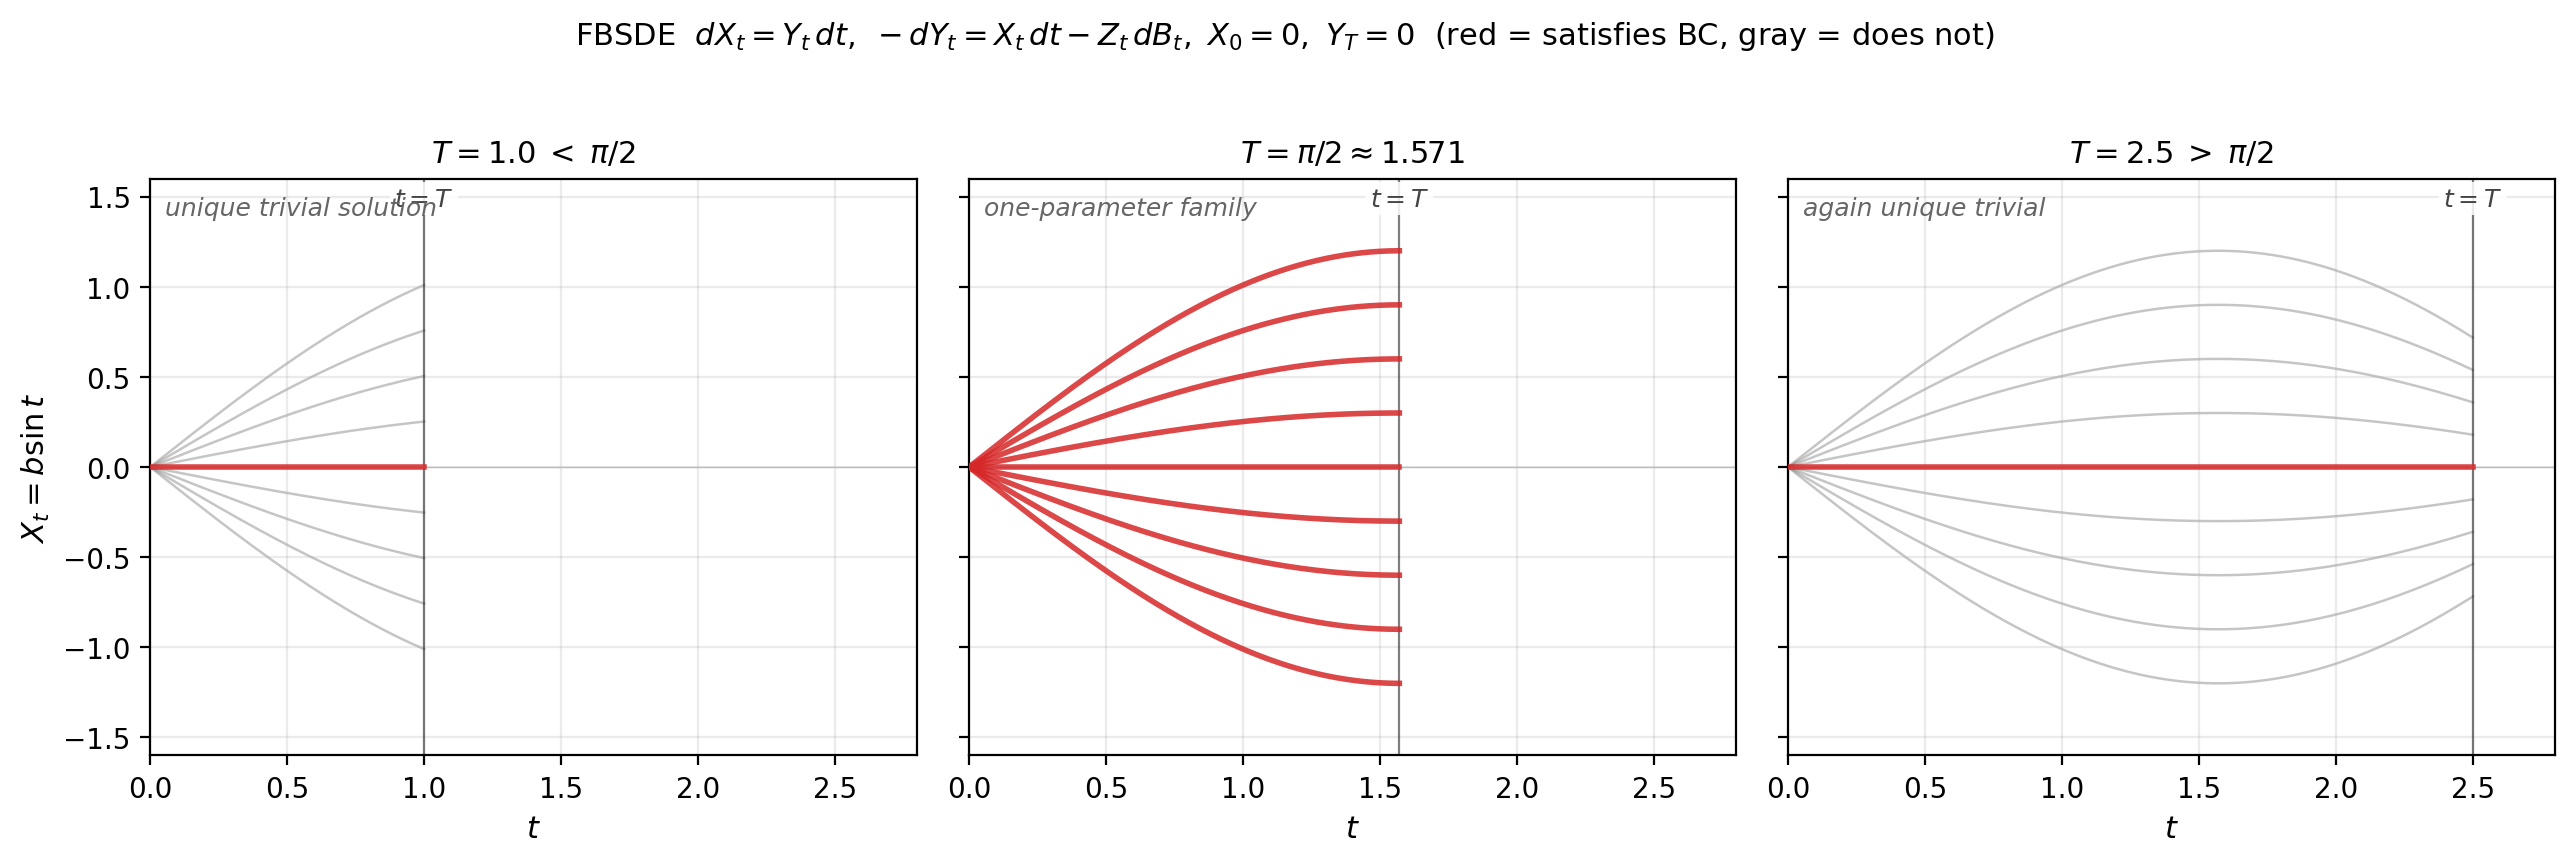
\includegraphics[width=\linewidth]{figures/fig1_antonelli.png}
\caption{Antonelli 的线性例子 \eqref{eq:antonelli}。对确定性族 $X_t=b\sin t$、$Y_t=b\cos t$，初始条件 $X_0=0$ 自动满足，终端条件 $Y_T=0$ 化为 $b\cos T=0$。红色曲线满足终端条件，灰色曲线不满足。左：$T=1<\pi/2$ 时，只有 $b=0$ 可行。中：$T=\pi/2$ 时，任何 $b$ 都可行，故唯一性失效。右：$T=2.5\in(\pi/2,3\pi/2)$ 时，又只有 $b=0$ 可行。因此该奇点是一种边值特征值现象，而非过了某个固定时间之后单调地丧失适定性。}
\label{fig:antonelli}
\end{figure}

\subsection{解耦场}

对 Markov 型 FBSDE，即系数逐点依赖于时间与过程、而非依赖于整条路径，一个关键启发是\textbf{解耦场}：一个函数
\[
  u:[0,T]\times\R^n\to\R^m,
\]
使得沿任意解都有
\[
  Y_t=u(t,X_t).
\]
若 $\sigma$ 不依赖 $Z$，并且 $u$ 足够光滑，则 It\^o 公式给出
\[
  Z_t=D_xu(t,X_t)\,\sigma(t,X_t,u(t,X_t)),
\]
其中 $D_xu$ 是 $m\times n$ 的 Jacobi 矩阵，因此 $D_xu\,\sigma$ 的维数正好是 $m\times d$。

若 $\sigma$ 依赖 $Z$，则关系变成隐式代数方程
\begin{equation}\label{eq:implicitZ}
  Z_t=D_xu(t,X_t)\,\sigma(t,X_t,u(t,X_t),Z_t).
\end{equation}
此时仅仅知道 $u$ 还不够，还要保证 \eqref{eq:implicitZ} 关于 $Z_t$ 可解且解唯一。

在最干净的情形下，即 $\sigma=\sigma(t,x)$，把 $Y_t=u(t,X_t)$ 和 $Z_t=D_xu(t,X_t)\sigma(t,X_t)$ 代回前向方程，得到
\[
  dX_t=b\bigl(t,X_t,u(t,X_t),D_xu(t,X_t)\sigma(t,X_t)\bigr)\,dt+\sigma(t,X_t)\,dB_t.
\]
于是 FBSDE 坍缩为仅关于 $X$ 的标准 SDE。若能找到 $u$，问题便被解耦。函数 $u$ 自身满足一个拟线性 PDE（见 \S4）。这正是四步格式的核心。

\section{单调性：Hu--Peng 方法}

要超越短视域，我们需要对系数施加一个代数条件，以阻止前向与倒向的误差互相放大。Hu 与 Peng 确定了一类这样的条件。为避免长方形矩阵的记账，我们先陈述一个强单调的方形版本：
\[
  X,Y\in\R^n,\qquad Z\in\R^{n\times d}.
\]
一般的 $G$-单调性条件类似，但在估计中使用 $G\Delta x$、$G^\top\Delta y$ 与 $G^\top\Delta z$，从而可以处理 $n\ne m$ 的情形。

对 $\theta=(x,y,z)$，定义带符号的系数向量
\[
  A(t,\theta):=\bigl(-f(t,\theta),\,b(t,\theta),\,\sigma(t,\theta)\bigr).
\]
符号的选取使得对 $\langle \Delta X_t,\Delta Y_t\rangle$ 应用 It\^o 公式时，漂移项恰好出现下面的内积。

\begin{definition}[强单调性]\label{def:monotone}
称系数 $(b,\sigma,f)$ 以常数 $\beta>0$ \textbf{强单调}，若对所有 $t$ 与所有 $\theta_1,\theta_2$，
\begin{equation}\label{eq:monotone}
  \bigl\langle A(t,\theta_1)-A(t,\theta_2),\theta_1-\theta_2\bigr\rangle\le-\beta |\theta_1-\theta_2|^2.
\end{equation}
这里第三个分量上的内积采用 Frobenius 内积。称终端映射与此单调性相容，若
\begin{equation}\label{eq:terminal}
  \langle g(x_1)-g(x_2),x_1-x_2\rangle\ge 0\qquad\text{对所有 }x_1,x_2\in\R^n.
\end{equation}
\end{definition}

\begin{remark}
条件 \eqref{eq:monotone} 是为了叙述简洁而采用的强版本。一般的 Hu--Peng 或 Peng--Wu 型条件允许不同分量有不同的耗散常数，也允许某些分量只通过满秩矩阵 $G$ 间接控制。强写成 $-\beta|\Delta\theta|^2$ 很干净，但会排除许多常见的 Hamilton 系统，例如扩散不依赖 $Z$ 的 LQ 问题。因此本节定理应理解为一个透明的充分条件，而不是最一般的形式。
\end{remark}

\begin{theorem}[Hu--Peng 型存在唯一性，强单调简化形式]\label{thm:hupeng}
设系数循序可测、关于 $(x,y,z)$ 一致 Lipschitz、具线性增长，并满足定义~\ref{def:monotone} 与终端相容性条件 \eqref{eq:terminal}。则对任意有限视域 $T>0$，FBSDE \eqref{eq:fbsde} 都有唯一解
\[
  (X,Y,Z)\in\Sc^2\times\Sc^2\times\Hc^2.
\]
\end{theorem}

\begin{proof}[证明（概要）]
所用技术是\textbf{连续性方法}。把 \eqref{eq:fbsde} 嵌入一族单参数系统 $(\Pi_\lambda)_{\lambda\in[0,1]}$，其中 $\Pi_0$ 取为一个简单可解的强单调 FBSDE，$\Pi_1$ 为目标系统。设
\[
  \Lambda=\{\lambda\in[0,1]:\Pi_\lambda\text{ 可解}\}.
\]
需证明：
\begin{enumerate}
  \item[(a)] $0\in\Lambda$；
  \item[(b)] 若 $\lambda\in\Lambda$，则 $\lambda+\varepsilon\in\Lambda$，其中 $\varepsilon>0$ 仅依赖于单调性常数与 Lipschitz 常数。
\end{enumerate}
步长一致正是单调性假设的要点所在。对两个候选三元组，记
\[
  \Delta X=X^1-X^2,\qquad \Delta Y=Y^1-Y^2,\qquad \Delta Z=Z^1-Z^2.
\]
将 It\^o 公式应用于 $\langle \Delta X_t,\Delta Y_t\rangle$，得到核心漂移项
\[
  \langle \Delta b,\Delta Y\rangle-\langle \Delta f,\Delta X\rangle+\langle \Delta\sigma,\Delta Z\rangle=\langle \Delta A,\Delta\theta\rangle.
\]
由强单调性，
\[
  \langle \Delta A,\Delta\theta\rangle\le-\beta|\Delta\theta|^2.
\]
另一方面，终端条件给出
\[
  \E\langle \Delta X_T,\Delta Y_T\rangle=\E\langle \Delta X_T,g(X_T^1)-g(X_T^2)\rangle\ge 0.
\]
两者合并产生先验估计，控制 $\Delta X,\Delta Y,\Delta Z$。这些估计使扰动映射在一个与 $\lambda$ 无关的小步长内成为压缩，因此连续性方法可以从 $\lambda=0$ 推到 $\lambda=1$。唯一性由同一估计直接给出。
\end{proof}

\begin{remark}[其他充分条件]
\hfill
\begin{itemize}
  \item Peng--Wu 将单调性型条件推广到任意视域上的随机 Hamilton 系统。
  \item Delarue 证明，当扩散非退化且不依赖 $(Y,Z)$ 时，PDE 方法可以给出另一条通往全局可解性的途径。
  \item Ma--Yong 的解耦场视角提供了一种系统方式，来整理连续性方法、四步格式与 PDE 方法之间的关系。
\end{itemize}
\end{remark}

\section{四步格式}

当系数足够正则，且某个 PDE 有古典解时，四步格式是 FBSDE 可解性最干净的构造性证明。它因构造的四个阶段而得名。

为使陈述透明，这里假设扩散是 Markov 型且不依赖倒向变量：
\[
  \sigma=\sigma(t,x).
\]
前向漂移仍可依赖 $(Y,Z)$。在此限制下，候选解耦场
\[
  u:[0,T]\times\R^n\to\R^m
\]
满足一个拟线性抛物型系统。

\subsection{四个步骤}

\paragraph{第 1 步：猜测解耦场。}
设存在
\[
  u\in C^{1,2}([0,T]\times\R^n;\R^m)
\]
使得 $Y_t=u(t,X_t)$。置
\[
  Z_t=D_xu(t,X_t)\sigma(t,X_t).
\]
It\^o 公式给出
\[
  dY_t=\left[\partial_tu+\frac12\operatorname{Tr}\bigl(\sigma\sigma^\top D^2_{xx}u\bigr)+D_xu\,b(t,X_t,u,Z_t)\right]dt+D_xu(t,X_t)\sigma(t,X_t)\,dB_t.
\]
因为 $u$ 是向量值函数，上式中的迹项按分量理解，即第 $i$ 个分量为
\[
  \operatorname{Tr}\bigl(\sigma\sigma^\top D^2_{xx}u^i\bigr).
\]
与
\[
  dY_t=-f(t,X_t,Y_t,Z_t)\,dt+Z_t\,dB_t
\]
比较，场 $u$ 必须求解
\begin{equation}\label{eq:quasilinear}
\begin{aligned}
  0={}&\partial_tu(t,x)+\frac12\operatorname{Tr}\bigl[\sigma\sigma^\top(t,x)D^2_{xx}u(t,x)\bigr] \\
  &+D_xu(t,x)\,b\bigl(t,x,u(t,x),D_xu(t,x)\sigma(t,x)\bigr) \\
  &+f\bigl(t,x,u(t,x),D_xu(t,x)\sigma(t,x)\bigr),
\end{aligned}
\end{equation}
终端条件为
\[
  u(T,x)=g(x).
\]

\paragraph{第 2 步：求解 PDE。}
在光滑性、有界性与一致抛物性假设下，古典抛物型 PDE 理论给出 \eqref{eq:quasilinear} 的古典解 $u$。这是分析上最困难的一步。

\paragraph{第 3 步：求解现已解耦的前向 SDE。}
有了 $u$，定义
\[
  \tilde b(t,x)=b\bigl(t,x,u(t,x),D_xu(t,x)\sigma(t,x)\bigr),
\]
并求解
\[
  dX_t=\tilde b(t,X_t)\,dt+\sigma(t,X_t)\,dB_t,\qquad X_0=x.
\]
这是一个标准 SDE。

\paragraph{第 4 步：读出 $(Y,Z)$。}
置
\[
  Y_t=u(t,X_t),\qquad Z_t=D_xu(t,X_t)\sigma(t,X_t).
\]
由第 1 步，$(X,Y,Z)$ 求解原 FBSDE。

\begin{theorem}[Ma--Protter--Yong，简化形式]\label{thm:mpy}
设 $b,\sigma,f,g$ 足够光滑且 Lipschitz，$\sigma\sigma^\top$ 一致椭圆，PDE \eqref{eq:quasilinear} 有至多多项式增长的古典解
\[
  u\in C^{1,2}.
\]
则在 $\sigma=\sigma(t,x)$ 下，第 3--4 步构造出的三元组 $(X,Y,Z)$ 是 FBSDE \eqref{eq:fbsde} 的平方可积解。唯一性至少在由该古典解耦场生成的 Markov 解类中成立；若再加上相应的全局适定性条件，例如单调性条件或小视域 Lipschitz 条件，则可得到平方可积解类中的唯一性。
\end{theorem}

\begin{figure}[htbp]
\centering
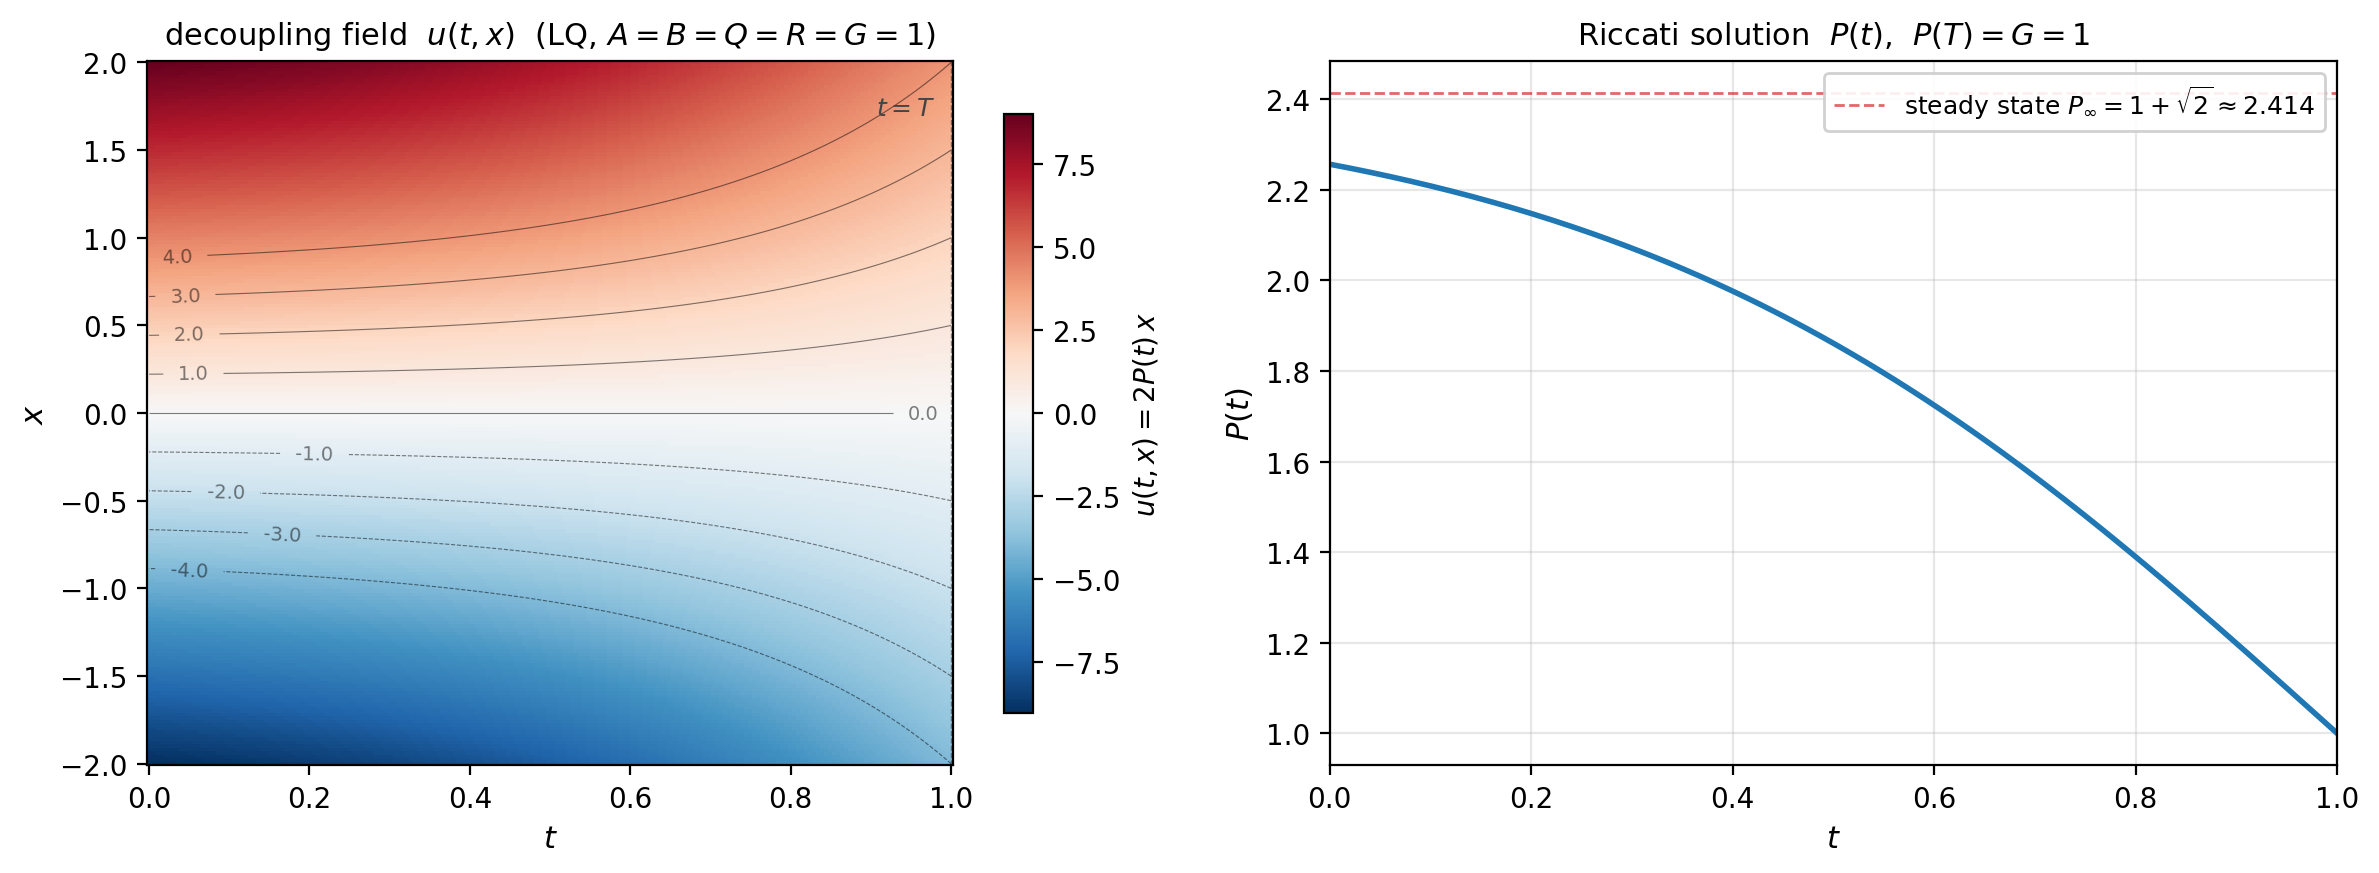
\includegraphics[width=\linewidth]{figures/fig2_decoupling_field.png}
\caption{取 $A=B=Q=R=G=1$、$T=1$ 的标量 LQ 问题的解耦场。左图绘出 $[0,1]\times[-2,2]$ 上的 $u(t,x)=2P(t)x$，这是当状态为 $X_t=x$ 时伴随变量 $Y_t$ 的值。右图绘出终端条件为 $P(T)=1$ 的 Riccati 解 $P(t)$。由于 $\dot P+2P-P^2+1=0$，有 $P(t)=1+\sqrt2\,\tanh\bigl(\sqrt2(1-t)\bigr)$。更长的倒向视域使 $P(t)$ 朝正的代数 Riccati 根 $1+\sqrt2$ 靠近。}
\label{fig:decoupling}
\end{figure}

\subsection{与非线性 Feynman--Kac 的关系}

[SDE~IV, 定理~5.1] 说过：半线性 PDE 的古典解 $u$ 通过置
\[
  Y_s=u(s,X_s),\qquad Z_s=D_xu(s,X_s)\sigma(s,X_s)
\]
产生 BSDE 的解。四步格式是其自然的\emph{耦合}推广：拟线性 PDE \eqref{eq:quasilinear} 的古典解通过同样的读出规则产生 FBSDE 三元组，附带的变化是 PDE 本身在其系数中含有 $u$ 与 $D_xu\,\sigma$。

\begin{remark}[当 PDE 没有古典解时]
四步格式要求第 2 步在古典意义下成功，这把它限制在一致抛物、系数光滑的情形。Delarue 展示了如何通过拟古典正则化将其推广到一些退化情形，而 \S3 的单调性方法覆盖了许多 PDE 只有弱解或粘性解的情形。
\end{remark}

\section{随机极大值原理}

我们现在把 FBSDE 与最优控制相连。为使陈述保持一阶，并避开控制进入扩散时出现的二阶伴随项，我们采用如下标准设定：
\begin{itemize}
  \item 状态 $X\in\R^n$，动力学为
  \[
    dX_t=b(t,X_t,\alpha_t)\,dt+\sigma(t,X_t)\,dB_t,\qquad X_0=x.
  \]
  \item 控制 $\alpha_t$ 取值于凸集 $A\subset\R^k$，且循序可测。
  \item 代价为
  \[
    J(\alpha)=\E\left[\int_0^T \ell(t,X_t,\alpha_t)\,dt+h(X_T)\right],
  \]
  待极小化。
\end{itemize}

\begin{definition}[Hamilton 量]\label{def:hamiltonian}
Hamilton 量为
\[
  H(t,x,y,z,a)=\langle b(t,x,a),y\rangle+\operatorname{tr}\bigl(\sigma^\top(t,x)z\bigr)+\ell(t,x,a),
\]
其中
\[
  a\in A,\qquad y\in\R^n,\qquad z\in\R^{n\times d}.
\]
\end{definition}

\subsection{原理}

\begin{theorem}[随机极大值原理，一阶形式]\label{thm:smp}
设 $\alpha^*$ 最优，$X^*$ 为对应状态。设 $b,\sigma,\ell,h$ 关于 $x$ 可微，$b,\ell$ 关于 $a$ 可微，并满足标准的可积性与正则性假设。则存在适应过程
\[
  (Y,Z)\in\Sc^2\times\Hc^2
\]
求解
\begin{equation}\label{eq:adjoint}
  -dY_t=\partial_x H(t,X_t^*,Y_t,Z_t,\alpha_t^*)\,dt-Z_t\,dB_t,\qquad Y_T=\partial_xh(X_T^*),
\end{equation}
使得对 $dt\otimes d\Prob$-几乎所有 $(t,\omega)$，
\begin{equation}\label{eq:vi}
  \bigl\langle\partial_aH(t,X_t^*,Y_t,Z_t,\alpha_t^*),\,a-\alpha_t^*\bigr\rangle\ge 0\qquad\text{对所有 }a\in A.
\end{equation}
若 $a\mapsto H(t,X_t^*,Y_t,Z_t,a)$ 凸，则 \eqref{eq:vi} 等价于
\begin{equation}\label{eq:argmin}
  \alpha_t^*\in\operatorname*{arg\,min}_{a\in A}H(t,X_t^*,Y_t,Z_t,a).
\end{equation}
\end{theorem}

因此 $(X^*,Y,Z)$ 连同反馈条件构成一个耦合的前向--倒向系统：状态决定伴随方程，而伴随决定最优反馈。

\begin{theorem}[充分条件，凸情形]\label{thm:sufficient}
设 $h$ 凸，且对每个 $(t,y,z)$，映射
\[
  (x,a)\longmapsto H(t,x,y,z,a)
\]
凸。若可行四元组 $(X^*,Y,Z,\alpha^*)$ 满足伴随方程 \eqref{eq:adjoint} 与逐点极小化条件 \eqref{eq:argmin}，则 $\alpha^*$ 最优。
\end{theorem}

\begin{proof}[证明（概要）]
对必要条件，取凸扰动
\[
  \alpha^\varepsilon=\alpha^*+\varepsilon(a-\alpha^*)
\]
并计算一阶变分 $\delta X$。伴随 BSDE 的选取恰好使得关于 $\langle Y_t,\delta X_t\rangle$ 的分部积分恒等式抵消 $J$ 的导数中的状态变分项。由于 $\alpha^*$ 极小化 $J$，剩下的一阶项对每个可行方向都非负，这便给出 \eqref{eq:vi}。

对充分条件，令 $\alpha$ 为任意可行控制，$X$ 为对应状态，并记
\[
  \Delta X_t=X_t-X_t^*,\qquad \Delta\alpha_t=\alpha_t-\alpha_t^*.
\]
由 $h$ 的凸性，
\[
  h(X_T)-h(X_T^*)\ge\langle h_x(X_T^*),\Delta X_T\rangle.
\]
再对 $\langle Y_t,\Delta X_t\rangle$ 使用 It\^o 公式，并代入伴随方程，可得
\[
\begin{aligned}
  J(\alpha)-J(\alpha^*)\ge\E\int_0^T\Big[&H(t,X_t,Y_t,Z_t,\alpha_t)-H(t,X_t^*,Y_t,Z_t,\alpha_t^*)\\
  &-\left\langle H_x(t,X_t^*,Y_t,Z_t,\alpha_t^*),\Delta X_t\right\rangle\Big]dt.
\end{aligned}
\]
由于 $H$ 对 $(x,a)$ 凸，
\[
\begin{aligned}
  &H(t,X_t,Y_t,Z_t,\alpha_t)-H(t,X_t^*,Y_t,Z_t,\alpha_t^*)-\left\langle H_x(t,X_t^*,Y_t,Z_t,\alpha_t^*),\Delta X_t\right\rangle\\
  &\qquad\ge\left\langle H_a(t,X_t^*,Y_t,Z_t,\alpha_t^*),\Delta\alpha_t\right\rangle,
\end{aligned}
\]
而逐点极小化条件给出右端非负。因此
\[
  J(\alpha)-J(\alpha^*)\ge 0.
\]
任意可行 $\alpha$ 皆如此，故 $\alpha^*$ 最优。
\end{proof}

\subsection{与 HJB 的对偶}

[SDE~IV, \S6.1] 给出了 HJB 途径：值函数
\[
  V(t,x)=\inf_\alpha\E\left[\int_t^T\ell(s,X_s,\alpha_s)\,ds+h(X_T)\,\Big|\,X_t=x\right]
\]
满足
\[
  \partial_tV+\inf_{a\in A}\tilde H(t,x,\partial_xV,\partial_{xx}V,a)=0,\qquad V(T,x)=h(x),
\]
其中动态规划 Hamilton 量为
\[
  \tilde H(t,x,p,M,a)=\langle b(t,x,a),p\rangle+\frac12\operatorname{Tr}\bigl(\sigma\sigma^\top(t,x)M\bigr)+\ell(t,x,a).
\]
若 $V\in C^{1,2}$，且 $\alpha^*$ 是最优反馈，则极大值原理中的伴随变量满足
\begin{equation}\label{eq:duality}
  Y_t=\partial_xV(t,X_t^*),\qquad Z_t=D^2_{xx}V(t,X_t^*)\,\sigma(t,X_t^*).
\end{equation}
因此 $Y$ 是值函数沿最优轨道的梯度，$Z$ 是由二阶空间导数与扩散矩阵生成的修正项。两种途径是对偶的：HJB 活在 PDE 一侧，极大值原理活在 FBSDE 一侧，而 \eqref{eq:duality} 把它们桥接起来。当 $V$ 光滑时，两种途径给出相同的答案；当 $V$ 仅为粘性解时，极大值原理往往更易应用，因为它不要求先验地知道值函数的二阶正则性。

\subsection{LQ 控制：详解例}

回到引言中的 LQ 问题：
\[
  dX_t=(AX_t+B\alpha_t)\,dt+\sigma\,dB_t,
\]
代价为
\[
  J(\alpha)=\E\!\left[\int_0^T\bigl(X_t^\top QX_t+\alpha_t^\top R\alpha_t\bigr)\,dt+X_T^\top GX_T\right],
\]
其中 $Q,G$ 对称半正定，$R\succ0$。Hamilton 量为
\[
  H(t,x,y,z,a)=\langle Ax+Ba,y\rangle+\operatorname{tr}(\sigma^\top z)+x^\top Qx+a^\top Ra.
\]
一阶条件 $\partial_aH=0$ 给出
\[
  \alpha_t^*=-\frac12R^{-1}B^\top Y_t.
\]
伴随 BSDE 为
\[
  -dY_t=(A^\top Y_t+2QX_t^*)\,dt-Z_t\,dB_t,\qquad Y_T=2GX_T^*.
\]
与受控状态 SDE 结合，得到线性 FBSDE：
\[
  \begin{cases}
    dX_t^*=\left(AX_t^*-\dfrac12BR^{-1}B^\top Y_t\right)dt+\sigma\,dB_t,\\[6pt]
    -dY_t=(A^\top Y_t+2QX_t^*)\,dt-Z_t\,dB_t,\\[3pt]
    X_0^*=x,\qquad Y_T=2GX_T^*.
  \end{cases}
\]
作拟设
\[
  Y_t=2P(t)X_t^*,
\]
其中 $P(t)$ 为确定性矩阵。代入伴随方程，则 $P$ 必须求解矩阵 Riccati 方程
\[
  \dot P+PA+A^\top P-PBR^{-1}B^\top P+Q=0,\qquad P(T)=G.
\]
在标准的矩阵条件下，$P$ 在 $[0,T]$ 上存在唯一。于是最优反馈为
\[
  \alpha_t^*=-R^{-1}B^\top P(t)X_t^*.
\]
这就是带时变增益的线性反馈。

\begin{remark}
通过 Pontryagin 与通过 HJB 来建立 LQ 问题，给出同一个 Riccati 方程。HJB 写出
\[
  V(t,x)=x^\top P(t)x+q(t)
\]
并代入；Pontryagin 写出
\[
  Y_t=2P(t)X_t^*
\]
并代入。两条路都碰到同一个非线性矩阵 ODE，因为 LQ 问题具有二次的值函数与线性的伴随。这是 \eqref{eq:duality} 可以手算验证的最简单情形。
\end{remark}

\begin{figure}[htbp]
\centering
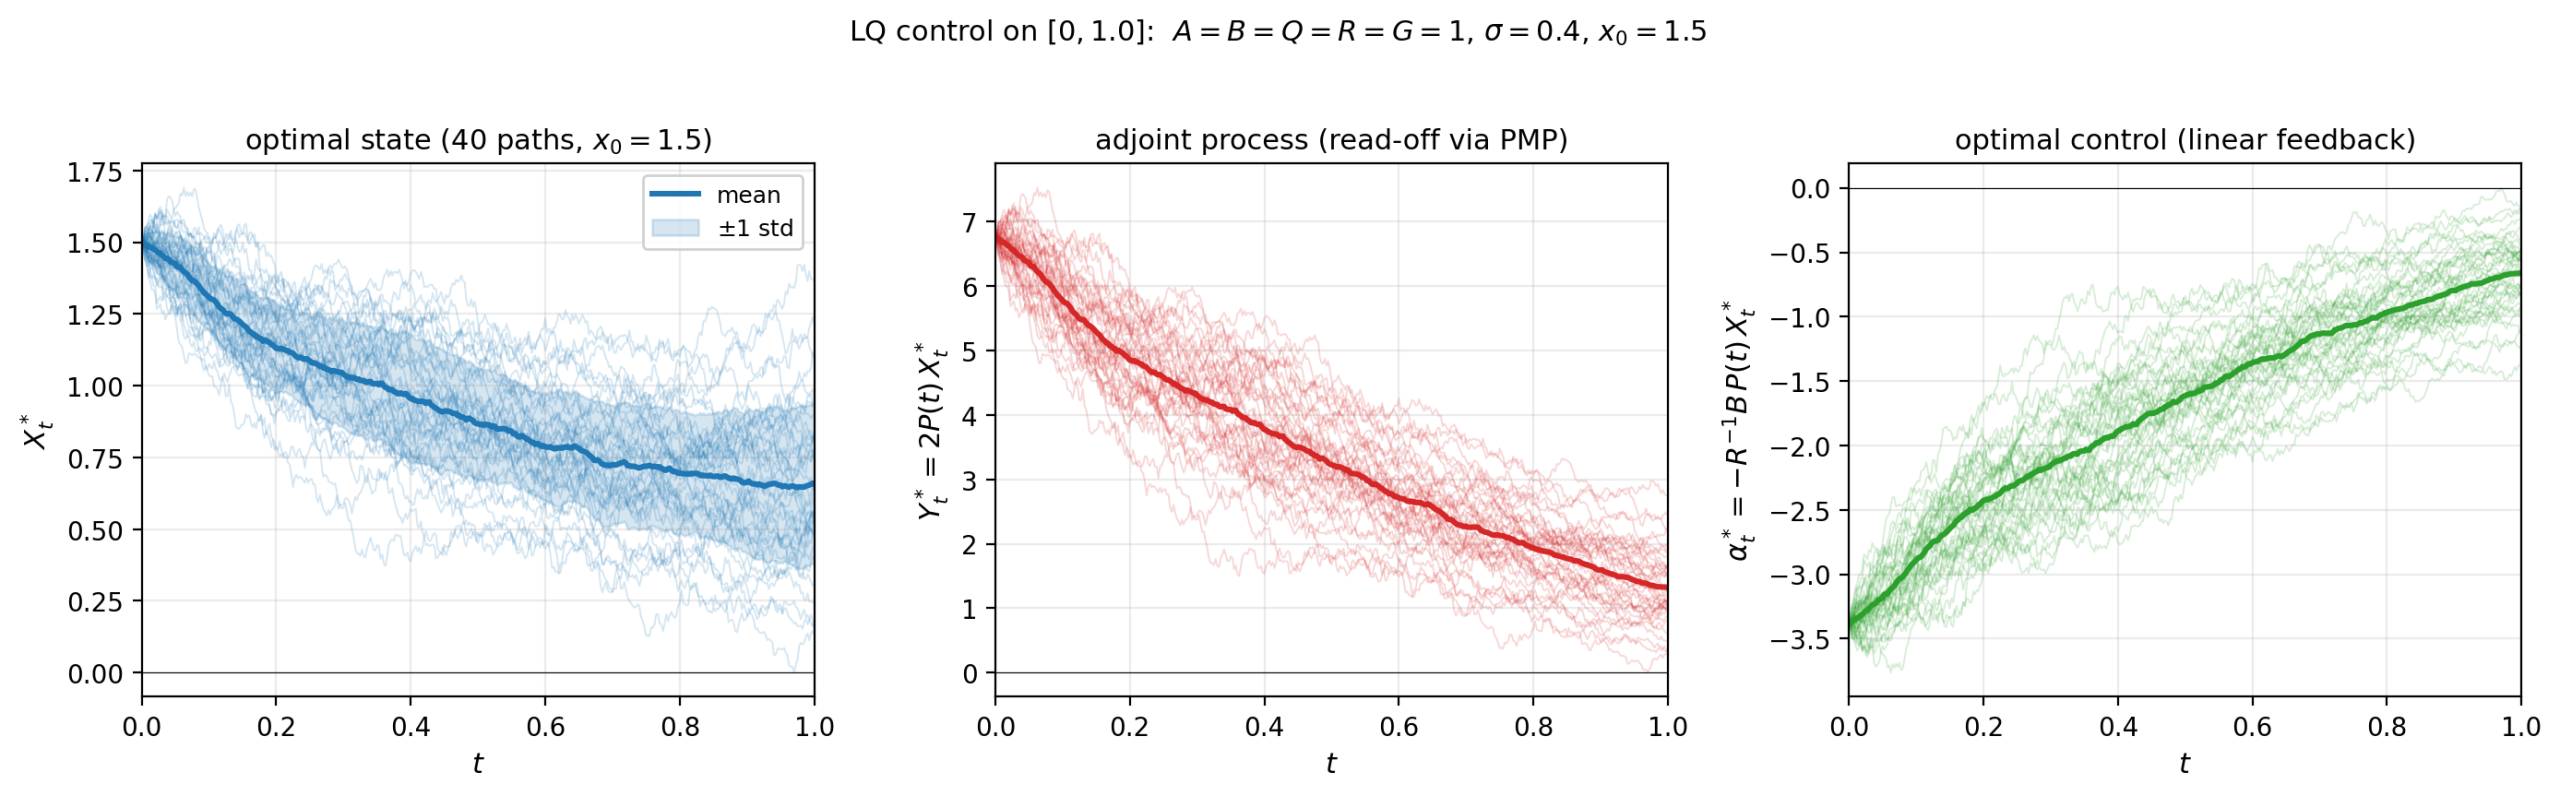
\includegraphics[width=\linewidth]{figures/fig3_lq_control.png}
\caption{取 $A=B=Q=R=G=1$、$\sigma=0.4$、$T=1$、$x_0=1.5$ 的闭环标量 LQ 控制，用 Euler--Maruyama 模拟。左图显示 $40$ 条 $X_t^*$ 的样本轨道以及均值 $\pm1$ 标准差包络。中图显示由极大值原理得到的伴随过程 $Y_t^*=2P(t)X_t^*$。右图显示反馈控制 $\alpha_t^*=-R^{-1}B^\top P(t)X_t^*$，它在 $t=0$ 附近强烈为负，并随状态趋近原点而松弛。其中的 Riccati 增益 $P(t)$ 与图~\ref{fig:decoupling} 中所绘的是同一个。}
\label{fig:lq}
\end{figure}

\section{应用}

\subsection{带约束的效用最大化}

考虑一位投资者，其终端财富 $W_T$ 由自融资投资组合生成：
\[
  dW_t=\pi_t\cdot\mu\,dt+\pi_t\cdot\sigma\,dB_t,\qquad W_0=w,
\]
其中 $\pi_t$ 是投在风险资产上的金额。投资者最大化
\[
  \E[U(W_T)],
\]
其中 $U$ 为凹效用，并受投资组合约束
\[
  \pi_t\in K,
\]
其中 $K$ 为闭凸集或闭凸锥。

无约束的 Merton 问题通常可以直接由 HJB 求解。带凸约束时，Cvitani\'c--Karatzas 的对偶方法引入一个取值于极约束集的对偶过程。原始财富方程与对偶鞅（或伴随方程）构成一个前向--倒向系统。确切的符号约定取决于把对偶变量放在状态价格密度的漂移里，还是放在 $K$ 的支撑函数里，但结构要点不变：前向财富过程与倒向边际效用过程通过互补松弛关系互相决定。在对偶定理的正则性与凸性假设下，这一 FBSDE 表述等价于带约束的最优投资问题，并在 $K=\R^d$ 时化归为 Merton 解。

\subsection{Deep FBSDE}

[SDE~IV, \S6.2] 的 Deep BSDE 方法自然地推广到耦合情形。将时间离散为
\[
  0=t_0<t_1<\cdots<t_M=T,\qquad \Delta t=T/M.
\]
参数化：
\begin{itemize}
  \item 初值 $Y_0=\theta_0\in\R^m$；
  \item 用每步一个神经网络逼近被积函数
  \[
    Z_k\approx z^\theta(t_k,X_{t_k}).
  \]
\end{itemize}
在第 $k$ 步，用当前估计
\[
  Y_{t_k},\qquad Z_{t_k}=z^\theta(t_k,X_{t_k})
\]
代入 $b,\sigma$，模拟
\[
  X_{t_{k+1}}=X_{t_k}+b(t_k,X_{t_k},Y_{t_k},Z_{t_k})\,\Delta t+\sigma(t_k,X_{t_k},Y_{t_k},Z_{t_k})\,\Delta B_k.
\]
再用 Euler 格式推进 $Y$：
\[
  Y_{t_{k+1}}=Y_{t_k}-f(t_k,X_{t_k},Y_{t_k},Z_{t_k})\,\Delta t+Z_{t_k}\Delta B_k.
\]
用随机梯度下降极小化终端失配
\[
  \mathcal J(\theta)=\E\bigl[|g(X_{t_M})-Y_{t_M}|^2\bigr].
\]
与 Deep BSDE 的关键区别是：在耦合情形中，$X$ 依赖于 $(Y,Z)$，所以前向链本身就含有可学习参数。

需要注意的是，在有限步 Euler 离散和有限网络类下，
\[
  \mathcal J(\theta)=0
\]
只表示离散终端条件被精确匹配。要从这个数值对象回到连续 FBSDE 的解，还需要控制时间离散误差、网络逼近误差与优化误差；在这些误差趋于零、并且连续 FBSDE 适定的条件下，Deep FBSDE 近似才可解释为收敛到连续解。

\subsection{关于耦合扩散的一点说明}

当 $\sigma$ 依赖于 $(Y,Z)$ 时，上面四步格式的干净版本不再直接适用。关系
\[
  Z=D_xu\,\sigma(t,x,u,Z)
\]
变成关于 $Z$ 的隐式代数方程。若该代数方程不可解或解不唯一，解耦场 $u$ 本身就不能直接生成 FBSDE 的解。即使该方程可解，相应的 PDE 也可能变为隐式的、强非线性的系统。

这与二阶 BSDE 有联系，但不能简单等同。更准确地说，2BSDE 通常出现在控制扩散、波动率不确定性、非支配测度族以及完全非线性 PDE 的概率表示中。Soner--Touzi--Zhang 的框架把这类二阶问题放入非线性期望与二阶倒向方程的理论中。耦合扩散的 FBSDE 有时会指向相似的完全非线性结构，但并非每个 $\sigma(Y,Z)$ 型 FBSDE 都自动是一个 2BSDE。

\section{展望}

\paragraph{反射型 FBSDE。}
像 [SDE~IV, \S7] 那样给倒向方程加一个下障碍 $L_t$，便得到反射型 FBSDE。它们出现在最优停时、奇异控制以及带约束的随机控制问题中。相应的 PDE 是带障碍的变分不等式。

\paragraph{平均场 FBSDE。}
让 $b,\sigma,f,g$ 依赖于边际律
\[
  \mathcal L(X_t),\qquad \mathcal L(Y_t),
\]
便导出平均场 FBSDE。它们是平均场博弈与平均场控制的自然状态方程形式。相应的 PDE，即\textbf{主方程}，定义在
\[
  [0,T]\times\R^n\times\mathcal P_2(\R^n)
\]
上，其存在唯一性理论目前非常活跃。

\paragraph{二阶 BSDE。}
如 \S6.3 所述，当扩散受控或存在波动率不确定性时，对偶对象往往是一个 2BSDE。它们以概率方式表示完全非线性 PDE。Soner--Touzi--Zhang 框架现在把 BSDE 与 2BSDE 统一在基于非线性期望的单一理论之下。

\paragraph{粗糙 BSDE 与粗糙 FBSDE。}
若驱动比半鞅情形更粗糙，则必须用粗糙路径或逐轨道随机分析取代 It\^o 微积分。这是一个更微妙、仍在发展的方向，因此最好与上面的布朗理论分开处理。

\begin{thebibliography}{99}
\bibitem{pp1990} Pardoux, E.; Peng, S. \emph{Adapted solution of a backward stochastic differential equation.} Systems \& Control Letters 14 (1990), 55--61.
\bibitem{antonelli} Antonelli, F. \emph{Backward--forward stochastic differential equations.} Annals of Applied Probability 3 (1993), 777--793.
\bibitem{mpy} Ma, J.; Protter, P.; Yong, J. \emph{Solving forward--backward stochastic differential equations explicitly: a four step scheme.} Probability Theory and Related Fields 98 (1994), 339--359.
\bibitem{hupeng} Hu, Y.; Peng, S. \emph{Solution of forward--backward stochastic differential equations.} Probability Theory and Related Fields 103 (1995), 273--283.
\bibitem{pengwu} Peng, S.; Wu, Z. \emph{Fully coupled forward--backward stochastic differential equations and applications to optimal control.} SIAM Journal on Control and Optimization 37 (1999), 825--843.
\bibitem{mayong} Ma, J.; Yong, J. \emph{Forward--Backward Stochastic Differential Equations and Their Applications.} Lecture Notes in Mathematics 1702, Springer, 1999.
\bibitem{yongzhou} Yong, J.; Zhou, X.~Y. \emph{Stochastic Controls: Hamiltonian Systems and HJB Equations.} Springer, 1999.
\bibitem{delarue} Delarue, F. \emph{On the existence and uniqueness of solutions to FBSDEs in a non-degenerate case.} Stochastic Processes and their Applications 99 (2002), 209--286.
\bibitem{ck} Cvitani\'c, J.; Karatzas, I. \emph{Convex duality in constrained portfolio optimization.} Annals of Applied Probability 2 (1992), 767--818.
\bibitem{stz} Soner, H.~M.; Touzi, N.; Zhang, J. \emph{Wellposedness of second order backward SDEs.} Probability Theory and Related Fields 153 (2012), 149--190.
\bibitem{hanlong} Han, J.; Long, J. \emph{Convergence of the deep BSDE method for coupled FBSDEs.} Probability, Uncertainty and Quantitative Risk 5, article 5 (2020), 1--33.
\bibitem{hpw} Hur\'e, C.; Pham, H.; Warin, X. \emph{Deep backward schemes for high-dimensional nonlinear PDEs.} Mathematics of Computation 89 (2020), 1547--1579.
\bibitem{cdll} Cardaliaguet, P.; Delarue, F.; Lasry, J.-M.; Lions, P.-L. \emph{The Master Equation and the Convergence Problem in Mean Field Games.} Princeton University Press, 2019.
\bibitem{lsu} Ladyzhenskaya, O.~A.; Solonnikov, V.~A.; Ural'tseva, N.~N. \emph{Linear and Quasi-linear Equations of Parabolic Type.} Translations of Mathematical Monographs 23, American Mathematical Society, 1968.
\bibitem{lieberman} Lieberman, G.~M. \emph{Second Order Parabolic Differential Equations.} World Scientific, 1996.
\end{thebibliography}

\clearpage % 在 CJK* 环境内输出最后一页（页眉含中文标题）
\end{CJK*}
\end{document}
